\documentclass[11pt]{article}

\usepackage[utf8]{inputenc}
\usepackage[T1]{fontenc}

\usepackage[a4paper, left=2cm, right=2cm, top=3.5cm, bottom=3.5cm]{geometry}
\usepackage[french]{babel}

% Paragraph spacing
\setlength{\parskip}{1em}

% Fancy headers
\usepackage{fancyhdr}

% Captions for subfigures
\usepackage{subcaption}


% Code highlighting
\usepackage{minted}

% Footnote inside a caption
\usepackage{fnpos}
\usepackage{ftnxtra}

% Colored text, provides \textcolor{color}{text}
\usepackage{xcolor}

% Maths
\usepackage{amsmath}
\usepackage{amssymb}

% Todo notes
\usepackage{todonotes}

% Table of contents for bibliography
\usepackage[nottoc]{tocbibind}

% Inline monospace font
\def\code#1{\texttt{#1}}

% Figures
\usepackage{graphicx}

% Draw figures
\usepackage{tikz}

% Code listing
\usepackage{listings}

% Tikz node rotation
\usetikzlibrary{positioning}

% Turing machine
\usetikzlibrary{chains,fit,shapes}

% Usage: \rotnode[options]{rotation}{text}
\newcommand\rotnode[3][]{%
\node [#1, opacity=0.0] (tmp) {#3};
\node [draw, rotate around={#2:(tmp.center)}] at (tmp) {#3};
}

% remove extra space
\newcommand{\squeezeup}{\vspace{-4.5cm}}

% Clickable links
\usepackage{hyperref}
% Table of contents depth
\setcounter{tocdepth}{2}

% Inline code
\usepackage{listings}
\usepackage{color}

\title{Systèmes d'exploitation - Moniteurs \& Sémaphores}

\author{Othmane AJDOR}
\date{2018-2019}

\begin{document}
\maketitle

\pagebreak
\tableofcontents
\pagebreak

\section{Philosophes}

\begin{figure}[h!]
    \centering
    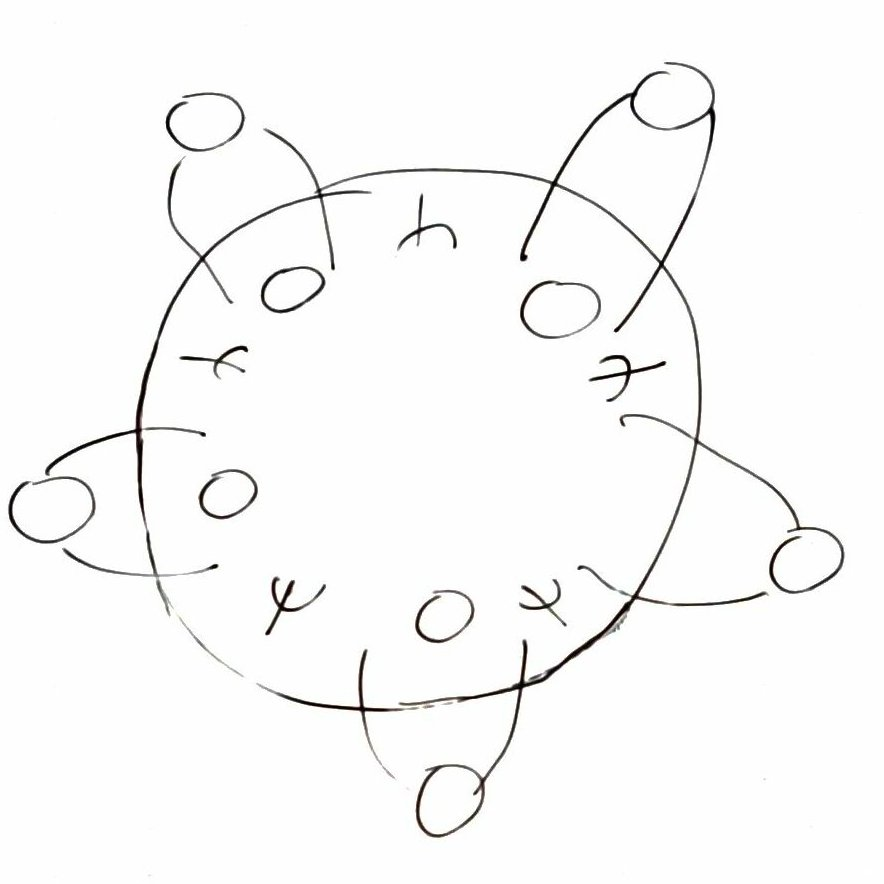
\includegraphics[scale=0.2]{img/RB_0131.jpg}
\end{figure}

\subsection{Moniteurs}
\begin{minted}[frame=single]{c}
    enum EtatPhilo{MANGE, PENSE};
    EtatPhilo etatsPhilo[N] = {PENSE, ...};
    mtx_t m;
    cnd_t prive[N];
    
    Philo(int i){
        while(1){
            pense();
            prendre_fourchette();
            mange();
            poser_fourchette();
        }
    }

    prendre_fourchettes(int i){
        mtx_lock(&m);
        int v1 = (i+N-1)%N;
        int v1 = (i+N+1)%N;
        while (etatsPhilo[v1] == MANGE || etatsPhilo[v2] == MANGE){
            cnd_wait(prive[i], &m);
        }
        etatsPhilo[i] = MANGE;
        mtx_unlock(&m);
    }

    poser_fourchettes(int i){
        mtx_lock(&m);
        etatsPhilo[i] = PENSE;
        int v1 = (i+N-1)%N;
        int v1 = (i+N+1)%N;
        cnd_signal(&prive[v1]);
        cnd_signal(&prive[v2]);
        mtx_inlock(&m);
    }
\end{minted}

\subsection{Dijkstra - Semaphore}

\begin{minted}[frame=single]{c}
    // Philo: un grand saladier de fourchettes + elastique => paire de fourchette
    int c; // Compteur
    sem_t s = N/2;

    Philo(int i){
        while(1){
            pense();
            prendre_fourchette();
            mange();
            poser_fourchette();
        }
    }

    // sem_wait()
    P(){
        c--;
        if (c<0){
            // mettre le thread en attente
        }
    }

    // sem_post()
    V(){
        c++;
        // debloquer un thread bloqué
        if(c <= 0)
    }

    poser_fouchettes(){
        V(&s);
    }
    prendre_fourchettes(){
        P(&s);
    }
\end{minted}

\pagebreak

Tous les philos ont pris la fourchette de droite
\begin{minted}[frame=single]{c}
    // PHILO 1 FAUX
    sem_t fourch[N] = {1,1...1};
    prendre_fourchettes(i){
        P(&fourch[i]);
        P(&fourch[(i+1)%N])
    }

    poser_fourchettes(i){
        V(&fourch[i]);
        V(&fourch[(i+1)%N]);
    }
\end{minted}

\begin{minted}[frame=single]{c}
    // PHILO 2 : 1 gaucher à choisir par le programmeur
    // N-1 au lieu de 0 pour prendre les ressources dans l'ordre pour eviter deadlock
    prendre_fourchette(i){
        if (i==N-1){ 
            P(&fourch[(i+1)%N]);
            P(&fourch[i]);
        } else {
            P(&fourch[i]);
            P(&fourch[(i+1)%N]);
        }
    }   

    poser_fourchette(i){
        V(&fourch[i]);
        V(&fourch[(i+1)%N]);
    } 
\end{minted}

\pagebreak

\begin{minted}[frame=single]{c}
    // PHILO 3: sas à N1
    sem_t sas = N - 1;
    prendre_fourchette(i){
        P(&sas);
        P(&fourch[i]);
        P(&fourch[(i+1)%N]);
        V(&sas);
    }

    poser_fourchette(i){
        V(&fourch[i]);
        V(&fourch[(i+1)%N]);
        V(&sas);
    }
\end{minted}

\begin{minted}[frame=single]{c}
    // Rendez-vous à 2
    sem_t nb_a = 0;
    sem_t nb_b = 0;

    arriveeA(){
        V(&nb_a);
        P(&nb_b);
    }

    arriveeB(){
        V(&nb_b);
        P(&nb_a);
    }
\end{minted}

\pagebreak

\begin{minted}[frame=single]{c}
    // Philo 4: 3 états
    enum EtatPhilo{MANGE, PENSE, AFAIM};
    EtatPhilo etatsPhilo[N] = {PENSE, ..., PENSE};
    sem_t sprive[N] = {0,..,0};
    sem_t ms = 1; // Exclusion mutuelle

    test(i){
        if (EtatPhilo[(i+1)%N] != MANGE && EtatPhilo[(i-1)%N] != MANGE 
                && EtatPhilo[i] == AFAIM){
            EtatPhilo[i] = MANGE;
            V(sprive[i]);
        }
    }

    prendre_fourchette(i){
        // (Changement d'état + test) en exclussion mutuelle 
        P(&ms);
        etatPhiio[i] = AFAIM;
        test(i);
        V(&ms);

        // Blocage
        P(&sprive[i]);
    }

    poser_fourchette(i){
        // En exclusion mutuelle
        P(&ms);
        etatPhilo[i] = PENSE;
        test((i+1)%N);
        test((i-1)%N);
        V(&ms);
    }
\end{minted}

\pagebreak

\subsection{Producteurs Consomateurs}
\begin{figure}[h!]
    \centering
    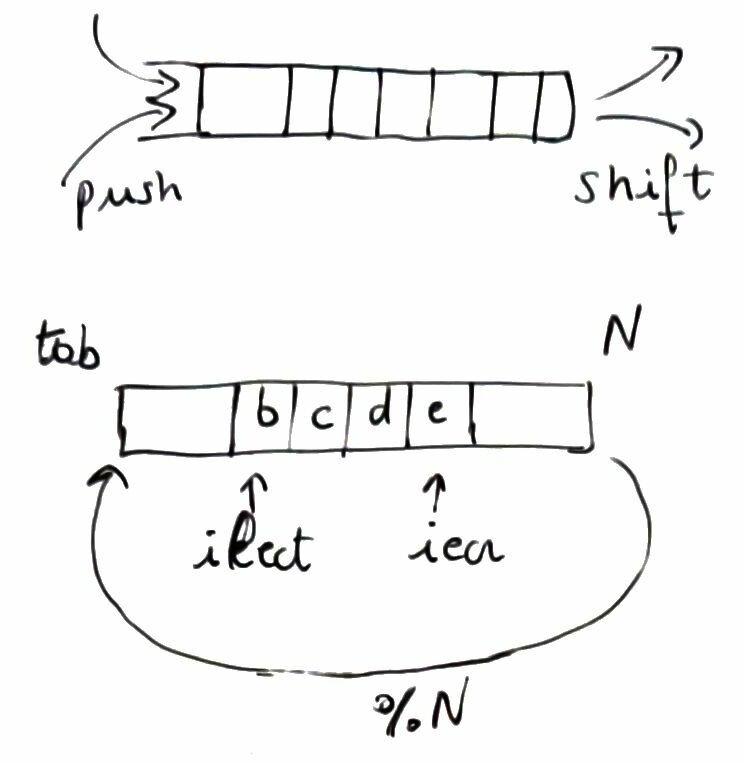
\includegraphics[scale=0.2]{img/prod_cons.jpg}
\end{figure}
\begin{minted}[frame=single]{c}
    sem_t ms = 1;
    sem_t pleines = 0;
    sem_t vides = N;
    int ilect, iecr;
    Tampon tab[N];

    push(Msg msg){
        // Verifie s'il existe des cas vide puis se mettre en exclu mut
        P(&vides);
        P(&ms)
        
        // Ecrire le msg
        tab[iecr] = msg;
        iecr++;
        iecr %= N;

        // Lacher l'exclu mut
        V(&ms);
        V(&pleines)
    }

    MsgShift(){
        P(&pleine);
        P(&ms);
        
        Msg msg = tab[ilect];
        ilect = (ilect+1)%N;

        V(&ms);
        V(&vide);
        return msg;
    }
\end{minted}

\pagebreak

\subsection{Producteurs consommateurs 2 (Lire/Ecrire en même temps)}
Utiliser deux semaphores qui permettent de lire et ecrire en même temps sans mélanger.

\begin{minted}[frame=single]{c}
    sem_t ms = 1;
    sem_t ms2 = 1;
    sem_t pleines = 0;
    sem_t vides = N;
    int ilect, iecr;
    Tampon tab[N];

    push(Msg msg){
        // Verifie s'il existe des cas vide puis se mettre en exclu mut
        P(&vides);
        P(&ms)
        
        // Ecrire le msg
        tab[iecr] = msg;
        iecr++;
        iecr %= N;

        // Lacher l'exclu mut
        V(&ms);
        V(&pleines)
    }

    MsgShift(){
        P(&pleine);
        P(&ms2);
        
        Msg msg = tab[ilect];
        ilect = (ilect+1)%N;

        V(&ms2);
        V(&vide);
        return msg;
    }
\end{minted}

\pagebreak

\subsection{Lecteurs redacteurs}
Le but est de pouvoir lire à plusieurs mais d'ecrire tout seul.
\begin{minted}[frame=single]{c}
    int nblect = 0;
    sem_t ms = 1;
    sem_t acces_BD = 1; // Acces à la base de données
    sem_t sas = 1; // FIFO aux redacteurs

    debut_lire(){
        P(&sas);
        P(&ms);
        nblect++;
        if (nblect == 1){
            P(&acces_BD);
        }
        V(&ms);
        V(&sas);
    }

    fin_lire(){
        P(&ms);
        nblect--;
        if (nblect == 0){
            V(&acces_BD);
        }
        V(&ms);
    }

    debut_ecr(){
        P(&sas);
        P(&acces_BD);
        V(&sas);
    }

    fin_ecr(){
        V(&acces_BD);
    }
\end{minted}

\end{document}